\documentclass[11pt,class=report,crop=false]{standalone}
\usepackage[screen]{../python}

\begin{document}

%====================================================================
\chapitre{Principales fonctions}
%====================================================================


%%%%%%%%%%%%%%%%%%%%%%%%%%%%%%%%%%%%%%%%%%%%%%%%%%%%
\section{Mathématiques}

\textbf{Opérations classiques}
\begin{itemize}
  \item \ci{a + b},\quad \ci{a - b},\quad \ci{a * b}\quad  opérations classiques
  \item \ci{a / b}\quad division \og{}réelle\fg{} (renvoie un nombre flottant)
  \item \ci{a // b}\quad quotient de la division euclidienne (renvoie un entier)
  \item \ci{a \% b}\quad reste de la division euclidienne, appelé $a$ modulo $b$
  \item \ci{abs(x)}\quad valeur absolue
  \item \ci{x ** n}\quad puissance $x^n$
  \item \ci{4.56e12}\quad pour $4.56 \times 10^{12}$
\end{itemize}

\bigskip

\textbf{Module \og{}math\fg{}}

L'usage d'autres fonctions mathématiques nécessite le recours au module \ci{math} qui s'appelle par la commande :
\mycenterline{\ci{from math import *}}

\begin{itemize}
  \item \ci{sqrt(x)}\quad racine carrée $\sqrt{x}$
  \item \ci{cos(x)},\quad \ci{sin(x)},\quad \ci{tan(x)}\quad fonctions trigonométriques $\cos x$, $\sin x$, $\tan x$ en radians
  \item \ci{pi}\quad valeur approchée de $\pi = 3.14159265\ldots$
  \item \ci{inf} \quad valeur $+\infty$ (plus grande que tout autre nombre flottant)
  \item \ci{-inf} \quad valeur $-\infty$ (plus petite que tout autre nombre flottant)  
  \item \ci{floor(x)}\quad  entier juste en-dessous de $x$
  \item \ci{ceil(x)}\quad  entier juste au-dessus de $x$
  \item \ci{gcd(a,b)}\quad pgcd de $a$ et de $b$
  \item \ci{exp(x)} \quad exponentielle $e^x$
  \item \ci{log(x)} \quad logarithme népérien (en base $e$), $\ln(x)$  
  \item \ci{log(x,b)} \quad logarithme de $x$ en base $b$, $\log_b(x)$
  \item \ci{log(x,10)} \quad logarithme décimal, $\log_{10}(x)$
  \item \ci{log(x,2)} \quad logarithme en base $2$, $\log_{2}(x)$
  \item \ci{acos(x)},\quad \ci{asin(x)},\quad \ci{atan(x)}\quad fonctions trigonométriques inverse $\arccos x$, $\arcsin x$, $\arctan x$, renvoie un angle en radians
  \item \ci{atan2(y,x)} \quad renvoie l'angle $\arctan(\frac yx)$ en radians. C'est l'angle entre l'horizontale et le vecteur $\overrightarrow{OM}$, où $M$ est le point de coordonnées $(x,y)$.
 \end{itemize}

\bigskip

\textbf{Nombres complexes}

Les nombres complexes sont compris nativement par \Python, cependant pour davantage de fonctionnalités on peut utiliser le module \ci{cmath}. Pour éviter les conflits avec le module \ci{math} on l'importe par :
\mycenterline{\ci{import cmath}}

\begin{itemize}
	\item \ci{z.real} \quad (sans parenthèses) partie réelle $a$ de $z=a+ib$
	\item \ci{z.imag} \quad (sans parenthèses) partie imaginaire $b$ de $z=a+ib$	 
	\item \ci{abs(z)} \quad module $|z| = \sqrt{a^2+b^2}$
	\item \ci{z.conjugate()} \quad conjugué $\bar z = a-ib$
	
	\item \ci{cmath.phase(z)} \quad argument $\theta \in ]-\pi,+\pi]$ de $z$
	
	\item \ci{cmath.rect(r,theta)}\index{rect@\ci{rect}} renvoie le nombre complexe dont le module est $r$ et l'argument $\theta$
 \end{itemize}


 \bigskip

\textbf{Module \og{}random\fg{}}

Le module \ci{random} génère des nombres de façon pseudo-aléatoire. Il s'appelle par la commande :
\mycenterline{\ci{from random import *}}

\begin{itemize}
  \item \ci{random()}\quad à chaque appel, renvoie un nombre flottant $x$ au hasard vérifiant  $0 \le x < 1$.
  \item \ci{randint(a,b)} \quad à chaque appel, renvoie un nombre entier $n$ au hasard vérifiant $a \le n \le b$.
  \item  \ci{choice(liste)} \quad à chaque appel, tire au hasard un élément de la liste.
  \item \ci{liste.shuffle()} \quad mélange la liste (la liste est modifiée).
 \end{itemize}

\bigskip

\textbf{\'Ecriture binaire}

\begin{itemize}
  \item \ci{bin(n)}\quad renvoie l'écriture binaire de l'entier $n$ sous la forme d'une chaîne. 
  Exemple : \ci{bin(17)} renvoie \ci{'0b10001'}.
  
  \item Pour écrire directement un nombre en écriture binaire, il suffit d'écrire le nombre en commençant par \ci{0b} (sans guillemets). Par exemple \ci{0b11011} vaut \ci{27}.
 \end{itemize}


\bigskip

\textbf{Affectation multiple}

\Python{} permet les affectations multiples, ce qui permet d'échanger facilement le contenu de deux variables.

\begin{itemize}
	\item \textbf{Affectation multiple.} 
	\mycenterline{\ci{a, b, c = 3, 4, 5}}
	Maintenant \ci{a} vaut $3$, \ci{b} vaut $4$ et \ci{c} vaut $5$.
	
	\item \textbf{\'Echange de valeurs.}	
	\mycenterline{\ci{a, b = b, a}}
	Maintenant \ci{a} vaut l'ancien contenu de \ci{b} donc vaut $4$ et \ci{b} vaut l'ancien contenu de \ci{a} donc $3$.
	
	\item \textbf{\'Echange à la main.} Pour échanger deux valeurs sans utiliser la double affectation, il faut introduire une variable temporaire :
\begin{lstlisting}		
temp = a
a = b
b = temp			
\end{lstlisting}
\end{itemize}

\emph{Note.} \Python{} est suffisamment intelligent pour autoriser une syntaxe souple, par exemple afin de passer d'une liste aux éléments de cette liste :
\begin{lstlisting}		
liste = [2,3,4]
a,b,c = liste	# a vaut 2, b vaut 3,...
\end{lstlisting}
Par contre lors d'un appel à une fonction il est nécessaire de décompacter (\emph{unpacking}) à l'aide de l'opérateur \og{}\ci{*}\fg{} utilisé en préfixe.
\begin{lstlisting}
def ma_fonction(a,b,c):
    ...
    
liste = [2,3,4]
ma_fonction(*liste) # note l'étoile ! 
\end{lstlisting}
L'instruction \ci{ma_fonction(*liste)} équivaut ici à l'appel \ci{ma_fonction(2,3,4)}.



\bigskip

\textbf{Incrémentation rapide}

Pour incrémenter une variable on écrit simplement :
\mycenterline{\ci{x = x + 1}}
mais on peut utiliser l'opérateur \og{}\ci{+=}\fg{} pour écrire  plus simplement :
\mycenterline{\ci{x += 1}}.

L'opérateur \og{}\ci{+=}\fg{} peut être utilisé dans d'autres situations :
\begin{itemize}
	\item \ci{x += 2} \quad pour \ci{x = x + 2}
	
	\item \ci{chaine += "mot"} \quad pour \ci{chaine = chaine + "mot"}
	
	\item\ci{liste += [element]} \quad pour \ci{liste = liste + [element]} ou \ci{liste.append(element)}	
\end{itemize}



\bigskip

\textbf{\'Evaluation}

\begin{itemize}
\item \ci{eval(chaine)} permet d'évaluer une expression donnée sous la forme d'une chaîne de caractères. 

\item Par exemple \ci{eval('8*3')} renvoie $24$.

\item Par exemple \ci{eval('2+2 == 2*2')} renvoie \ci{True}.
\end{itemize}


%%%%%%%%%%%%%%%%%%%%%%%%%%%%%%%%%%%%%%%%%%%%%%%%%%%%
\section{Booléens}

Un booléen est une donnée qui prend soit la valeur \ci{True} (\og{}Vrai\fg{}), soit la valeur \ci{False} (\og{}Faux\fg{}).

  
\bigskip

\textbf{Comparaisons}
 
Les tests de comparaison suivants renvoient un booléen.
  \begin{itemize}
    \item \ci{a == b} \quad test d'égalité
    	\item \ci{a < b} \quad test inférieur strict
    	\item \ci{a <= b} \quad test inférieur large
    	\item \ci{a > b} \quad ou \quad \ci{a >= b}\quad test supérieur
    	\item \ci{a != b} \quad test de non égalité
  \end{itemize}
  
 Ne pas confondre \og{}\ci{a = b}\fg{} (affectation) et \og{}\ci{a == b}\fg{} (test d'égalité).
  
\bigskip
  
\textbf{Opérations sur les booléens}
  \begin{itemize}
    \item \ci{P and Q} \quad \og{}et\fg{} logique
    	\item \ci{P or Q} \quad \og{}ou\fg{} logique
    	\item \ci{not P} \quad négation
  \end{itemize} 
  
  
%%%%%%%%%%%%%%%%%%%%%%%%%%%%%%%%%%%%%%%%%%%%%%%%%%%%
\section{Chaînes de caractères I}

\textbf{Chaînes}

\begin{itemize}
  \item \ci{"A"} \quad ou\quad \ci{'A'} \quad un caractère
  \item \ci{"Python"}\quad ou\quad \ci{'Python'} \quad une chaîne de caractères
  \item \ci{len(chaine)}\quad la longueur de la chaîne. Exemple : \ci{len("Python")} renvoie $6$.
  \item \ci{chaine1 + chaine2}\quad concaténation. 
  
  Exemple : \ci{"J aime bien" + "Python"} renvoie \ci{"J aime bienPython"}.
  
  \item \ci{chaine[i]}\quad renvoie le $i$-ème caractère de \ci{chaine} (la numérotation commence à $0$). 
  
  Exemple avec \ci{chaine = "Python"}, \ci{chaine[1]} vaut \ci{"y"}. Voir le tableau ci-dessous.
\end{itemize}

\begin{center}
\begin{tabular}{|c||c|c|c|c|c|c|}
\hline
Lettre & \textbf{P} & \textbf{y} & \textbf{t} & \textbf{h} & \textbf{o} & \textbf{n} \\ \hline
Rang & 0 & 1 & 2 & 3 & 4 & 5 \\ \hline
\end{tabular}
\end{center}


\textbf{Conversion nombre/chaîne}

\begin{itemize}
  \item \textbf{Chaîne.} \ci{str(nombre)}\quad convertit un nombre (entier ou flottant) en une chaîne.
  Exemples : \ci{str(7)} renvoie la chaîne \ci{"7"} ; \ci{str(1.234)} renvoie la chaîne \ci{"1.234"}.
  
  \item \textbf{Entier.} \ci{int(chaine)}\quad renvoie l'entier correspondant à la chaîne. Exemple \ci{int("45")} renvoie l'entier \ci{45}.
  
   \item \textbf{Nombre flottant.} \ci{float(chaine)}\quad renvoie le nombre flottant correspondant à la chaîne. Exemple \ci{float("3.14")} renvoie le nombre \ci{3.14}. 
 \end{itemize}  


\bigskip

\textbf{Sous-chaînes}

\begin{itemize}
  \item \ci{chaine[i:j]}\quad renvoie la sous-chaîne des caractères de rang $i$ à $j-1$ de \ci{chaine}.
  
   Exemple : avec \ci{chaine = "Ceci est une chaine"}, \ci{chaine[2:6]} renvoie \ci{"ci e"}.
   
  \item \ci{chaine[i:]}\quad renvoie les caractères de rang $i$ jusqu'à la fin de \ci{chaine}. 
  
  Exemple :
  \ci{chaine[5:]} renvoie \ci{"est une chaine"}.
  
  \item\ci{chaine[:j]}\quad renvoie les caractères du début jusqu'au rang $j-1$ de \ci{chaine}. Exemple :
  \ci{chaine[:4]} renvoie \ci{"Ceci"}.
  
\end{itemize}


\bigskip
\textbf{Mise en forme}

La méthode \ci{format()} permet de mettre en forme du texte ou des nombres. Cette fonction renvoie une chaîne de caractères.

\begin{itemize}
  \item \textbf{Texte}
  
  \begin{center}
 \lstinline[showspaces=true]!Test      ! \qquad\qquad
    \lstinline[showspaces=true]!      Test!  \qquad\qquad
 \lstinline[showspaces=true]!   Test   !   
 \end{center}
 
  \begin{itemize}
    \item \ci{'\{:10\}'.format('Test')} \quad alignement à gauche (sur 10 caractères)
    \item \ci{'\{:>10\}'.format('Test')} \quad alignement à droite
    \item \ci{'\{:\^10\}'.format('Test')} \quad centré 
  \end{itemize}

  \item \textbf{Entier}
  
  \begin{center}
 \lstinline[showspaces=true]!456! \qquad\qquad
    \lstinline[showspaces=true]!   456!  \qquad\qquad
 \lstinline[showspaces=true]!000456!   
 \end{center}
 
  \begin{itemize}
    \item \ci{'\{:d\}'.format(456)} \quad entier  
    \item \ci{'\{:6d\}'.format(456)} \quad alignement à droite (sur 6 caractères)
    \item \ci{'\{:06d\}'.format(456)} \quad ajout de zéros non significatifs  (sur 6 caractères)
  \end{itemize} 
  
  \item \textbf{Nombre flottant}
  
  \begin{center}
 \lstinline[showspaces=true]!3.141593! \qquad\qquad
    \lstinline[showspaces=true]!3.14159265!  \qquad\qquad
 \lstinline[showspaces=true]!  3.1416!  \qquad\qquad
 \lstinline[showspaces=true]!003.1416!   
 \end{center}
 
  \begin{itemize}
    \item \ci{'\{:f\}'.format(3.141592653589793)} \quad nombre flottant 
    \item \ci{'\{:.8f\}'.format(3.141592653589793)} \quad $8$ chiffres après la virgule 
    \item \ci{'\{:8.4f\}'.format(3.141592653589793)} \quad sur $8$ caractères avec $4$ chiffres après la virgule 
    \item 
    \ci{'\{:08.4f\}'.format(3.141592653589793)} \quad ajout de zéros non significatifs 
  \end{itemize}   
   
\end{itemize}



%%%%%%%%%%%%%%%%%%%%%%%%%%%%%%%%%%%%%%%%%%%%%%%%%%%%
\section{Chaînes de caractères II}



\textbf{Encodage}

\begin{itemize}
  \item \ci{chr(n)} \quad renvoie le caractère associé au numéro de code ASCII/unicode $n$. Exemple : \ci{chr(65)} renvoie \ci{"A"} ; \ci{chr(97)} renvoie \ci{"a"}.
    
  \item \ci{ord(c)} \quad renvoie le numéro de code ASCII/unicode associé au caractère $c$. Exemple : \ci{ord("A")} renvoie \ci{65} ; \ci{ord("a")} renvoie \ci{97}.
\end{itemize}

Le début de la table des codes ASCII/unicode est donné ci-dessous.

\myfigure{0.8}{
\small
  \tikzinput{chaines-unicode}
} 

\bigskip

\textbf{Majuscules/minuscules}

\begin{itemize}
  \item \ci{chaine.upper()} renvoie une chaîne en majuscules.
  \item \ci{chaine.lower()} renvoie une chaîne en minuscules.  
\end{itemize}

\bigskip

\textbf{Chercher/remplacer}

\begin{itemize}
  \item \ci{sous_chaine in chaine} \quad renvoie \og{}vrai\fg{} ou \og{}faux\fg{} si \ci{sous_chaine} apparaît dans \ci{chaine}.
  
   Exemple :
\ci{"PAS" in "ETRE OU NE PAS ETRE"} vaut \ci{True}.

  \item  \ci{chaine.find(sous_chaine)} \quad renvoie le rang auquel  la sous-chaîne a été trouvée (et \ci{-1} sinon).
  
  Exemple : avec \ci{chaine = "ABCDE"}, \ci{chaine.find("CD")} renvoie  \ci{2}.
  
   \item  \ci{chaine.replace(sous_chaine,nouv_sous_chaine)} \quad remplace 
   chaque occurrence de la sous-chaîne par la nouvelle sous-chaîne.
   
   Exemple : avec \ci{chaine = "ABCDE"}, \ci{chaine.replace("CD","XY")} renvoie
   \ci{"ABXYE"}.
   
   \item \ci{ligne.strip()}\index{strip@\ci{strip}} renvoie la chaîne de caractères de la ligne sans les espaces de début et de fin, ni le saut de ligne. 
   
   Exemple : avec \ci{ligne = " Il était une fois ! \\n"}, \ci{ligne.strip()} renvoie
   \ci{'Il était une fois !'}.

\end{itemize}


\bigskip

\textbf{Séparer/regrouper}

\begin{itemize}
  \item \ci{chaine.split(separateur)} \quad sépare la chaîne en une liste de sous-chaînes (par défaut le séparateur est l'espace).
  
  Exemples : 
  \begin{itemize}  
    \item \ci{"Etre ou ne pas etre.".split()} \quad renvoie \ci{['Etre', 'ou', 'ne', 'pas', 'etre.']}
    \item \ci{"12.5;17.5;18".split(";")} \quad renvoie \ci{['12.5', '17.5', '18']}
  \end{itemize}   
  
   \item \ci{separateur.join(liste)} \quad regroupe les sous-chaînes en une seule chaîne en ajoutant le séparateur entre chaque.

   Exemples :
  \begin{itemize}  
    \item \ci{"".join(["Etre", "ou", "ne", "pas", "etre."])} \quad renvoie \ci{'Etreounepasetre.'} Il manque les espaces.
    \item \ci{" ".join(["Etre", "ou", "ne", "pas", "etre."])} \ renvoie \ci{'Etre ou ne pas etre.'}   C'est mieux lorsque le séparateur est une espace.
    \item \ci{"--".join(["Etre", "ou", "ne", "pas", "etre."])}  renvoie
    
        \ci{'Etre--ou--ne--pas--etre.'}  
  \end{itemize} 
  
  

\end{itemize}


%%%%%%%%%%%%%%%%%%%%%%%%%%%%%%%%%%%%%%%%%%%%%%%%%%%%
\section{Listes I}

\textbf{Construction d'une liste}

Exemples :
\begin{itemize}
    \item \ci{liste1 = [5,4,3,2,1]} \quad une liste de $5$ entiers.
    \item \ci{liste2 = ["Vendredi","Samedi","Dimanche"]} \quad une liste de $3$ chaînes.
    \item \ci{liste3 = []} \quad la liste vide.
    \item \ci{list(range(n))} \quad liste des entiers de $0$ à $n-1$.
    \item \ci{list(range(a,b))} \quad liste des entiers de $a$ à $b-1$.
    \item \ci{list(range(a,b,saut))} \quad liste des entiers de $a$ à $b-1$, avec un pas donné par l'entier \ci{saut}.
  \end{itemize}
  
\bigskip
 
\textbf{Accéder à un élément}

\begin{itemize}
    \item \ci{liste[i]} \quad renvoie l'élément de la liste de rang $i$. Attention, le rang commence à $0$.

Exemple :  \ci{liste = ["A","B","C","D","E","F"]} alors \ci{liste[2]} renvoie \ci{"C"}.

\medskip
 \begin{center}
\begin{tabular}{|c||c|c|c|c|c|c|}
\hline
Lettre & \textbf{"A"} & \textbf{"B"} & \textbf{"C"} & \textbf{"D"} & \textbf{"E"} & \textbf{"F"} \\ \hline
Rang & 0 & 1 & 2 & 3 & 4 & 5 \\ \hline
\end{tabular}
\end{center}
\medskip

    \item \ci{liste[-1]} \quad renvoie le dernier élément, \ci{liste[-2]} renvoie l'avant-dernier élément\ldots
    
    
    \item \ci{liste.pop()} \quad supprime le dernier élément  de la liste et le renvoie (c'est l'opération \og{}dépiler\fg{}).
\end{itemize}


\bigskip

\textbf{Ajouter un élément (ou plusieurs)} 

\begin{itemize}

    \item \ci{liste.append(element)} \quad ajoute l'élément à la fin de la liste.
    Exemple : si \ci{liste = [5,6,7,8]} alors 
  \ci{liste.append(9)} rajoute $9$ à la liste, \ci{liste} vaut \ci{[5,6,7,8,9]}.
  
    \item \ci{nouv_liste = liste + [element]} \quad fournit une nouvelle liste avec un élément en plus à la fin. Exemple : \ci{[1,2,3,4] + [5]} vaut \ci{[1,2,3,4,5]}.
    \item \ci{[element] + liste} \quad renvoie une liste où l'élément est ajouté au début. Exemple : \ci{[5] + [1,2,3,4]} vaut \ci{[5,1,2,3,4]}. 
     \item \ci{liste1 + liste2} \quad concatène les deux listes. 
     Exemple : avec \ci{liste1 = [4,5,6]} et \ci{liste2 = [7,8,9]} alors \ci{liste1 + liste2} vaut \ci{[4,5,6,7,8,9]}.
\end{itemize}

\bigskip

\textbf{Exemple de construction.} Voici comment construire la liste qui contient les premiers carrés :
   \begin{center}
  \begin{minipage}{0.9\textwidth}
\begin{lstlisting}
liste_carres = []          # On part d'un liste vide
for i in range(10):
    liste_carres.append(i**2)   # On ajoute un carré
\end{lstlisting}
  \end{minipage}
  \end{center}  
\`A la fin \ci{liste_carres} vaut :
\mycenterline{\ci{[0, 1, 4, 9, 16, 25, 36, 49, 64, 81]}}  


\bigskip
\textbf{Parcourir une liste} 

\begin{itemize}
  \item \ci{len(liste)} \quad renvoie la longueur de la liste. Exemple :  \ci{len([5,4,3,2,1])} renvoie $5$.
    
  \item  Parcourir simplement une liste (et ici afficher chaque élément) :
\begin{lstlisting}
for element in liste:
    print(element)
\end{lstlisting}

  \item Parcourir une liste à l'aide du rang.
\begin{lstlisting}
n = len(liste)
for i in range(n):
    print(i,liste[i])
\end{lstlisting}  
\end{itemize}


\bigskip
\textbf{Copier une liste} 
\begin{lstlisting}
new_list = list(liste)
\end{lstlisting}

%%%%%%%%%%%%%%%%%%%%%%%%%%%%%%%%%%%%%%%%%%%%%%%%%%%%
\section{Listes II}



\textbf{Mathématiques}

   \begin{itemize}
    \item \ci{max(liste)} \quad renvoie le plus grand élément. Exemple : \ci{max([10,16,13,14])} renvoie \ci{16}.
    
    \item \ci{min(liste)} \quad renvoie le plus petit élément. Exemple : \ci{min([10,16,13,14])} renvoie \ci{10}.
    
    \item \ci{sum(liste)}\quad renvoie la somme de tous les éléments. Exemple : \ci{sum([10,16,13,14])} renvoie \ci{53}.
\end{itemize}

\bigskip
    
\textbf{Trancher des listes}
  
  \begin{itemize}
    \item \ci{liste[a:b]} \quad renvoie la sous-liste des éléments du rang $a$ au rang $b-1$.
    
    \item \ci{liste[a:]} \quad renvoie la liste des éléments du rang $a$ jusqu'à la fin.
      
    \item \ci{liste[:b]} \quad renvoie la liste des éléments du début jusqu'au rang $b-1$.
    

\end{itemize}


\medskip
 \begin{center}
\begin{tabular}{|c||c|c|c|c|c|c|c|}
\hline
Lettre & \textbf{"A"} & \textbf{"B"} & \textbf{"C"} & \textbf{"D"} & \textbf{"E"} & \textbf{"F"} & \textbf{"G"} \\ \hline
Rang & 0 & 1 & 2 & 3 & 4 & 5 & 6 \\ \hline
\end{tabular}
\end{center}
\medskip
  
    Par exemple si \ci{liste = ["A","B","C","D","E","F","G"]} alors :
  \begin{itemize}
    \item \ci{liste[1:4]} \quad renvoie \ci{["B","C","D"]}.
    \item \ci{liste[:2]} \quad c'est comme \ci{liste[0:2]} et renvoie \ci{["A","B"]}.   
    \item \ci{liste[4:]} \quad renvoie \ci{["E","F","G"]}.  C'est la même chose 
     que \ci{liste[4:n]} où \ci{n = len(liste)}.
  \end{itemize} 

\bigskip

\textbf{Trouver le rang d'un élément} 

\begin{itemize}

    \item   
   \ci{liste.index(element)} renvoie la première position à laquelle l'élément a été trouvé. Exemple : avec \ci{liste = [12, 30, 5, 9, 5, 21]},
   \ci{liste.index(5)} renvoie $2$.

  \item Si on souhaite juste savoir si un élément appartient à une liste, alors l'instruction :  
  \mycenterline{\ci{element in liste}}  
  renvoie \ci{True} ou \ci{False}.
  Exemple : avec \ci{liste = [12, 30, 5, 9, 5, 21]},
   \og\ci{9 in liste}\fg{} est vrai, alors que \og\ci{8 in liste}\fg{} est faux.
  
\end{itemize}

\bigskip

\textbf{Ordonner}

\begin{itemize}
  \item \ci{sorted(liste)} \quad  renvoie la liste ordonnée des éléments.
  
   Exemple : \ci{sorted([13,11,7,4,6,8,12,6])} renvoie la liste \ci{[4,6,6,7,8,11,12,13]}.
   
   \item \ci{liste.sort()} \quad  ne renvoie rien mais par contre la liste \ci{liste} est maintenant ordonnée.
\end{itemize}


\bigskip

\textbf{Inverser une liste}

Voici trois méthodes :
\begin{itemize}
  \item \ci{liste.reverse()} \quad modifie la liste sur place ;
  \item \ci{list(reversed(liste))} \quad  renvoie une nouvelle liste ;
  \item \ci{liste[::-1]} \quad renvoie une nouvelle liste. 
\end{itemize}  


\bigskip

\textbf{Supprimer un élément}

Trois méthodes.
\begin{itemize}
  \item  \ci{liste.remove(element)} \quad supprime la première occurrence trouvée.
  
   Exemple : \ci{liste = [2,5,3,8,5]}, la commande \ci{liste.remove(5)} modifie la liste qui maintenant vaut \ci{[2,3,8,5]} (le premier $5$ a disparu).
  
   \item \ci{del liste[i]} \quad supprime l'élément de rang $i$ (la liste est modifiée).
   
   \item \ci{element = liste.pop()} \quad supprime le dernier élément de la liste et le renvoie. C'est l'opération \og{}dépiler\fg{}.
\end{itemize}


\bigskip

\textbf{Liste par compréhension}

  \begin{itemize}
    \item Partons d'une liste, par exemple \ci{maliste = [1,2,3,4,5,6,7,6,5,4,3,2,1]}.
    
    \item \ci{liste_doubles = [ 2*x for x in maliste ]} \quad renvoie une liste qui contient les doubles des éléments de la liste \ci{maliste}. C'est donc la liste 
    \ci{[2,4,6,8,...]}.
    
    \item \ci{liste_carres = [ x**2 for x in maliste ]} \quad renvoie la liste des carrés de éléments de la liste \ci{maliste}. C'est donc la liste \ci{[1,4,9,16,...]}.
    
    \item \ci{liste_partielle = [x for x in maliste if x > 2]} \quad
    extrait la liste composée des seuls éléments strictement supérieurs à $2$. C'est donc la liste \ci{[3,4,5,6,7,6,5,4,3]}.
	\end{itemize}
	
\bigskip	 

\textbf{Liste de listes}
  
Exemple : 
  \mycenterline{\ci{tableau = [ [2,14,5], [3,5,7], [15,19,4], [8,6,5] ]}}
  correspond au tableau :
  \myfigure{0.7}{
  \tikzinput{fig-tableau}
}
  Alors \ci{tableau[i]} renvoie la sous-liste de rang $i$, et
  \ci{tableau[i][j]} renvoie l'élément situé dans la sous-liste de rang $i$, au rang $j$ de cette sous-liste. Par exemple :
  \begin{itemize}
  \item \ci{tableau[0]} \quad renvoie la sous-liste \ci{[2,14,5]}.
  \item \ci{tableau[1]} \quad renvoie la sous-liste \ci{[3,5,7]}.
  \item \ci{tableau[0][0]} \quad renvoie l'entier \ci{2}.
  \item \ci{tableau[0][1]} \quad renvoie l'entier \ci{14}.
  \item \ci{tableau[2][1]} \quad renvoie l'entier \ci{19}.
\end{itemize}

\medskip

Un tableau de $n$ lignes et $p$ colonnes.
\begin{itemize}
    \item \ci{tableau = [[0 for j in range(p)] for i in range(n)]} \quad initialise un tableau et le remplit de $0$.
    \item \ci{tableau[i][j] = 1} \quad modifie une valeur du tableau (celle à l'emplacement $(i,j)$).
\end{itemize}

%%%%%%%%%%%%%%%%%%%%%%%%%%%%%%%%%%%%%%%%%%%%%%%%%%%%
\section{Dictionnaire}

Un dictionnaire est un peu comme une liste, mais les éléments ne sont pas indexés par des entiers mais par une \og{}clé\fg{}. Un \defi{dictionnaire} est donc un ensemble de couples clé/valeur : à une \defi{clé} est associée une \defi{valeur}.

\medskip

\textbf{Exemple : un dictionnaire identifiant/mot de passe.}

\begin{itemize}
	\item Voici l'exemple d'un dictionnaire \ci{dico} qui stocke des identifiants et des mots de passe : 
	\mycenterline{\ci{dico = \{'jean':'rev1789', 'adele':'azerty', 'jasmine':'c3por2d2'\}}}
	
	\item Par exemple \ci{'adele'} a pour mot de passe \ci{'azerty'}. On obtient le mot de passe
	comme on accéderait à un élément d'une liste par l'instruction :
	\mycenterline{\ci{dico['adele']} \quad qui vaut\quad \ci{'azerty'}.}
	
	\item Pour ajouter une entrée on écrit : 
	\mycenterline{\ci{dico['lola'] = 'abcdef'}}
	
	\item Pour modifier une entrée : 
	\mycenterline{\ci{dico['adele'] = 'vwxyz'}}
	
	\item Maintenant la commande \ci{print(dico)} affiche :
	\mycenterline{\ci{\{'jean':'rev1789', 'adele':'vwxyz', 'jasmine':'c3por2d2', 'lola':'abcdef'\}}}
	
	\item Le parcours d'un dictionnaire se fait par une boucle \og{}pour\fg{}. Par exemple, la boucle suivante affiche l'identifiant et le login de tous les éléments du dictionnaire :
	\begin{lstlisting}
	for prenom in dico:
	    print(prenom + " a pour mot de passe " + dico[prenom])
	\end{lstlisting}
	
	\item Attention : il n'y a pas d'ordre dans un dictionnaire. Tu ne contrôles pas dans quel ordre les éléments sont traités.
\end{itemize}

\medskip

\textbf{Commandes principales.}

\begin{itemize}
	\item Définir un dictionnaire \ci{dico = \{cle1:valeur1, cle2:valeur2,...\}}
	
	\item Récupérer une valeur : \ci{dico[cle]}
	
	\item Ajouter une valeur : \ci{dico[new_cle] = valeur}
	
	\item Modifier une valeur : \ci{dico[cle] = new_valeur}
	
	\item Taille du dictionnaire : \ci{len(dico)}
	
	\item Parcourir un dictionnaire : \ci{for cle in dico:} et dans la boucle on accède aux valeurs par \ci{dico[cle]}
	
	\item Tester si une clé existe : \ci{if cle in dico:}
	
	\item Dictionnaire vide : \ci{dico = \{\}}, utile pour initialiser un dictionnaire dans le but de le remplir ensuite.
\end{itemize}  

\bigskip

Des commandes un peu moins utiles :
\begin{itemize}
	
	\item Liste des clés : \ci{dico.keys()}\index{keys@\ci{keys}}
	
	\item Liste des valeurs : \ci{dico.values()}\index{values@\ci{values}}
	
	\item On peut récupérer les clés et les valeurs pour les utiliser dans une boucle :
	\begin{lstlisting}
	for cle,valeur in dico.items():
	    print("Clé :", cle, " Valeur :", valeur)
	\end{lstlisting}
\end{itemize}


%%%%%%%%%%%%%%%%%%%%%%%%%%%%%%%%%%%%%%%%%%%%%%%%%%%%
\section{Entrée/sortie}

\textbf{Affichage}

\begin{itemize}
  \item \ci{print(chaine1,chaine2,chaine3,...)} \quad affiche des chaînes ou des objets.
 Exemple : \ci{print("Valeur =",14)} affiche \ci{Valeur = 14}.
 Exemple : \ci{print("Ligne 1 \\n Ligne 2")} affiche sur deux lignes.
 
  \item \textbf{Séparateur.} \ci{print(...,sep="...")} \quad change le séparateur (par défaut le séparateur est le caractère espace). Exemple : \ci{print("Bob",17,13,16,sep="; ")} affiche
  \ci{Bob; 17; 13; 16}.
  
   \item \textbf{Fin de ligne.} \ci{print(...,end="...")} \quad change le caractère placé à la fin (par défaut c'est le saut de ligne \ci{\\n}).
   Exemple \ci{print(17,end="")} puis \ci{print(89)} affiche \ci{1789} sur une seule ligne.
   
\end{itemize}

\bigskip

\textbf{Entrée clavier}

\ci{input()} \quad  met le programme en pause et attend de l'utilisateur un message au clavier (qu'il termine en appuyant sur la touche \og{}Entrée\fg{}). Le message est une chaîne de caractères.

Voici un petit programme qui demande le prénom et l'âge de l'utilisateur et affiche un message du style 
\og{}Bonjour Kevin\fg{} puis \og{}Tu es mineur/majeur\fg{} selon l'âge. 
\begin{lstlisting}
prenom = input("Comment t'appelles-tu ? ")
print("Bonjour",prenom)

age_chaine = input("Quel âge as-tu ? ")
age = int(age_chaine)

if age >= 18:
    print("Tu es majeur !")
else:
    print("Tu es mineur !")
\end{lstlisting}  




%%%%%%%%%%%%%%%%%%%%%%%%%%%%%%%%%%%%%%%%%%%%%%%%%%%%
\section{Fichiers}

\textbf{Commande} 

\begin{itemize}
  \item \ci{fic = open("mon_fichier.txt","r")} \quad ouverture en lecture (\ci{"r"} = \emph{read}).
  \item \ci{fic = open("mon_fichier.txt","w")} \quad ouverture en écriture (\ci{"w"} = \emph{write}). Le fichier est créé s'il n'existe pas, s'il existait le contenu précédent est d'abord effacé.
  \item \ci{fic = open("mon_fichier.txt","a")} \quad ouverture en écriture, les données seront écrites à la fin des données actuelles (\ci{"a"} = \emph{append}).
  
  \item \ci{fic.write("une ligne")} \quad écriture dans le fichier.
  \item \ci{fic.read()} \quad lit tout le fichier (voir plus bas pour autre méthode).
  \item \ci{fic.readlines()} \quad lit toutes les lignes (voir plus bas pour autre méthode).
  
  \item \ci{fic.close()} \quad fermeture du fichier.
\end{itemize}

\bigskip

\textbf{\'Ecrire des lignes dans un fichier} 

\begin{lstlisting}
fic = open("mon_fichier.txt","w")

fic.write("Bonjour le monde\n")

ligne = "Coucou\n"
fic.write(ligne)

fic.close()
\end{lstlisting}



\bigskip

\textbf{Lire les lignes d'un fichier} 

\begin{lstlisting}
fic = open("mon_fichier.txt","r")

for ligne in fic:
    print(ligne)

fic.close()
\end{lstlisting}

\emph{Utile.} La commande \ci{ligne.strip()}\index{strip@\ci{strip}} renvoie la chaîne de caractères de la ligne sans les espaces de début et de fin, ni le saut de ligne. 

\bigskip

\textbf{Lire un fichier (méthode officielle)} 

\begin{lstlisting}
with open("mon_fichier.txt","r") as fic: 
    for ligne in fic: 
        print(ligne) 
\end{lstlisting}


%%%%%%%%%%%%%%%%%%%%%%%%%%%%%%%%%%%%%%%%%%%%%%%%%%%%
\section{Tortue}

Le module \ci{turtle} s'appelle par la commande :
\mycenterline{\ci{from turtle import *}}

\bigskip

\textbf{Principales commandes}
\begin{itemize}
  \item \ci{forward(longueur)} \quad avance de \ci{longueur} pas
  \item \ci{backward(longueur)} \quad recule
  \item \ci{right(angle)} \quad tourne vers la droite selon l'angle donné en degrés
  \item \ci{left(angle)} \quad tourne vers la gauche
  \item \ci{setheading(direction)} \quad s'oriente dans une direction ($0$ = droite, $90$ = haut, $-90$ = bas, $180$ = gauche)
  \item \ci{goto(x,y)} \quad se déplace jusqu'au point $(x,y)$
  \item \ci{setx(newx)} \quad change la valeur de l'abscisse (déplacement horizontal)
  \item \ci{sety(newy)} \quad change la valeur de l'ordonnée (déplacement vertical)
  
  
  \item \ci{down()} \quad abaisse le stylo
  \item \ci{up()} \quad relève le stylo
  \item \ci{width(epaisseur)} \quad change l'épaisseur du trait
  \item \ci{color(couleur)} \quad change la couleur du trait : \ci{"red"}, \ci{"green"}, \ci{"blue"}, \ci{"orange"}, \ci{"purple"},\ldots
  
  \item \ci{position()}  \quad renvoie la position $(x,y)$ de la tortue
  \item \ci{heading()} \quad renvoie la direction \ci{angle} vers laquelle pointe la tortue
  \item \ci{towards(x,y)} \quad renvoie l'angle entre l'horizontale et le segment commençant à la tortue et finissant au point $(x,y)$
  \item \ci{speed("fastest")} \quad vitesse maximale de déplacement
  \item \ci{hideturtle()} \quad cache le curseur de la tortue
  \item \ci{showturtle()} \quad affiche le curseur de la tortue  
  \item \ci{exitonclick()} \quad termine le programme dès que l'on clique
\end{itemize}

\bigskip

\textbf{Plusieurs tortues}

Voici un exemple de programme avec deux tortues.
\begin{lstlisting}
tortue1 = Turtle()   # Avec un 'T' majuscule !
tortue2 = Turtle()

tortue1.color('red')
tortue2.color('blue')

tortue1.forward(100)
tortue2.left(90)
tortue2.forward(100)
\end{lstlisting}



%%%%%%%%%%%%%%%%%%%%%%%%%%%%%%%%%%%%%%%%%%%%%%%%%%%%
\section{Matplotlib}

Avec le module \ci{matplotlib} il est très facile de tracer une liste. Voici un exemple.

\begin{center}
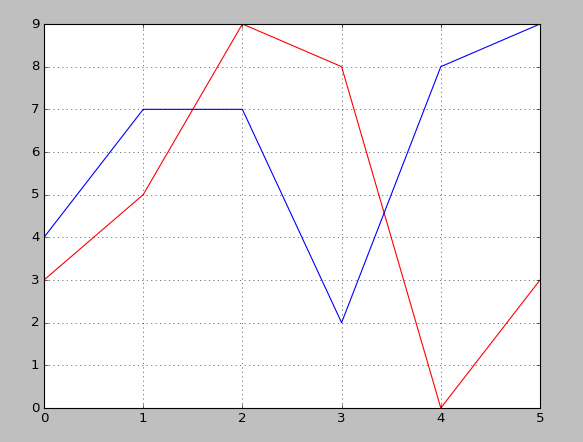
\includegraphics[scale=\myscale,scale=0.5]{ecran-liste-cours-visualisation}
\end{center}

\begin{lstlisting}
import matplotlib.pyplot as plt

liste1 = [3,5,9,8,0,3]
liste2 = [4,7,7,2,8,9]

plt.plot(liste1,color="red")
plt.plot(liste2,color="blue")
plt.grid()
plt.show()
\end{lstlisting}


\textbf{Principales fonctions.}

\begin{itemize}
  \item \ci{plt.plot(liste)} trace les points d'une liste (sous la forme $(i,\ell_i)$) et les joint. 
  \item \ci{plt.plot(listex,listey)} trace les points d'une liste (sous la forme $(x_i,y_i)$ où $x_i$ parcourt la première liste et $y_i$ la seconde).    
  \item \ci{plt.scatter(x,y,color='red',s=100)} affiche un point en $(x,y)$ (d'une grosseur \ci{s}).
  \item \ci{plt.grid()} trace une grille.  
  \item \ci{plt.show()} affiche tout. 
  \item \ci{plt.close()} termine le tracé.
  
  \item \ci{plt.xlim(xmin,xmax)} définit l'intervalle des $x$.
  \item \ci{plt.ylim(ymin,ymax)} définit l'intervalle des $y$.
  \item \ci{plt.axis('equal')} impose un repère orthonormé.  
\end{itemize}


%%%%%%%%%%%%%%%%%%%%%%%%%%%%%%%%%%%%%%%%%%%%%%%%%%%%
\section{Matplotlib 3D}

Avec le module \ci{matplolib} il est aussi assez facile de tracer une représentation des objets dans l'espace.
Le principe est similaire à l'affichage dans le plan, sauf bien sûr qu'il faut préciser trois coordonnées $x,y,z$ pour déterminer un point de l'espace.

\bigskip

Voici un code très simple qui affiche :
\begin{itemize}
	\item un point \couleurnb{bleu }{} de coordonnées $(2,1,3)$,
	\item des segments \couleurnb{rouges }{} qui relient les points de la liste  $(0,0,0)$, $(1,2,3)$, $(4,5,6)$, $(3,5,0)$.
\end{itemize}

\begin{center}
	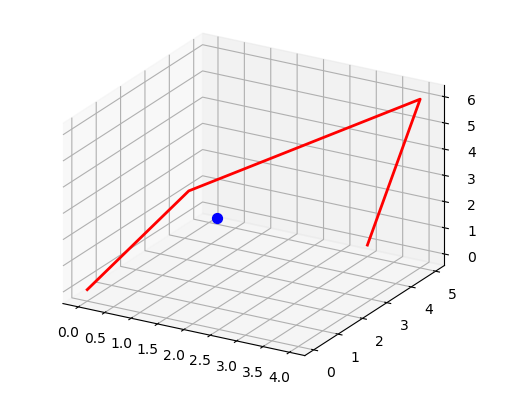
\includegraphics[scale=\myscale,scale=0.3]{../images3d/ecran-images3d-cours1}
	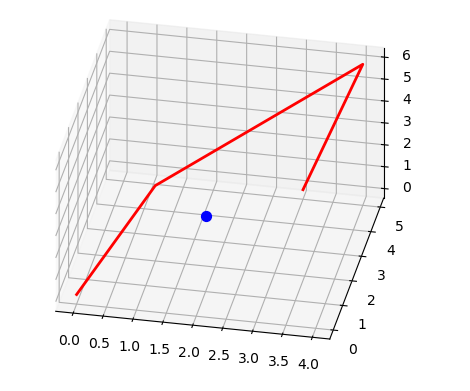
\includegraphics[scale=\myscale,scale=0.3]{../images3d/ecran-images3d-cours2}
	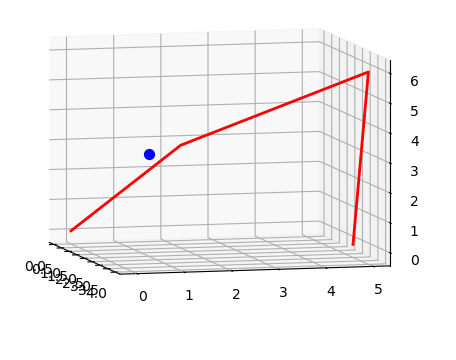
\includegraphics[scale=\myscale,scale=0.3]{../images3d/ecran-images3d-cours3}	
\end{center}

Une fenêtre s'affiche dans laquelle sont dessinés le point et les segments ainsi que les plans quadrillés de coordonnées. L'image est dynamique : à l'aide de la souris tu peux faire tourner le dessin afin de changer de point de vue.

\begin{lstlisting}
import matplotlib.pyplot as plt
from mpl_toolkits.mplot3d import Axes3D

# Initialisation
fig = plt.figure()
ax = fig.gca(projection='3d',proj_type = 'ortho') 

# Affichage d'un point
x,y,z = (2,1,3)
ax.scatter(x,y,z,color='blue',s=50)

# Segments reliant des points
points  = [(0,0,0),(1,2,3),(4,5,6),(3,5,0)]
liste_x = [x for x,y,z in points]
liste_y = [y for x,y,z in points]
liste_z = [z for x,y,z in points]

ax.plot(liste_x,liste_y,liste_z,color='red',linewidth=2)

# Affichage
plt.show()
\end{lstlisting}


\emph{Avertissement.} Pour afficher des segments la commande \ci{plot} n'est pas très naturelle (mais c'était déjà le cas dans le plan). Par exemple pour relier le point $(1,2,3)$ au point $(4,5,6)$ on donne d'abord la liste des $x$, puis la liste des $y$, puis la liste des $z$ :
\mycenterline{\ci{plot([1,4],[2,5],[3,6])}}

%%%%%%%%%%%%%%%%%%%%%%%%%%%%%%%%%%%%%%%%%%%%%%%%%%%%
\section{Tkinter}


Pour afficher ceci :
\begin{center}
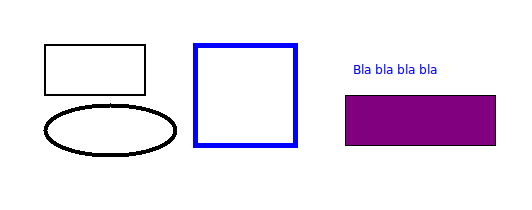
\includegraphics[scale=\myscale,scale=0.6]{ecran-stat-cours-intro}
\end{center}
le code est :
\begin{lstlisting}
# Module tkinter
from tkinter import *

# Fenêtre tkinter
root = Tk()
        
canvas = Canvas(root, width=800, height=600, background="white")
canvas.pack(fill="both", expand=True)

# Un rectangle
canvas.create_rectangle(50,50,150,100,width=2)

# Un rectangle à gros bords bleus
canvas.create_rectangle(200,50,300,150,width=5,outline="blue")

# Un rectangle rempli de violet
canvas.create_rectangle(350,100,500,150,fill="purple")

# Un ovale
canvas.create_oval(50,110,180,160,width=4)

# Du texte
canvas.create_text(400,75,text="Bla bla bla bla",fill="blue")

# Ouverture de la fenêtre
root.mainloop()
\end{lstlisting}


Quelques explications :
\begin{itemize}
  \item Le module \ci{tkinter} nous permet de définir des variables \ci{root} et \ci{canvas} qui définissent une fenêtre graphique (ici de largeur $800$ et de hauteur $600$ pixels).
  On décrit ensuite tout ce que l'on veut ajouter dans la fenêtre. Et enfin, la fenêtre est affichée par la commande \ci{root.mainloop()} (tout à la fin). 
  
    
  \item Attention ! Le repère graphique de la fenêtre a son axe des ordonnées dirigé vers le bas. L'origine $(0,0)$ est le coin en haut à gauche (voir la figure ci-dessous). 
  
  \item Commande pour tracer un rectangle : \ci{create_rectangle(x1,y1,x2,y2)} ; il suffit de préciser les coordonnées $(x_1,y_1)$ et $(x_2,y_2)$ de deux sommets opposés. L'option \ci{width} ajuste l'épaisseur du trait, \ci{outline} définit la couleur de ce trait et \ci{fill} définit la couleur de remplissage.
  
  \item Une ellipse est tracée par la commande \ci{create_oval(x1,y1,x2,y2)}, où $(x_1,y_1)$, $(x_2,y_2)$ sont les coordonnées de deux sommets opposés d'un rectangle encadrant l'ellipse voulue (voir la figure). On obtient un cercle lorsque le rectangle correspondant est un carré.  
  
  \item Le texte est affiché par la commande \ci{canvas.create_text()} en précisant les coordonnées $(x,y)$ du point à partir duquel on souhaite afficher le texte. 
  
\end{itemize}

\myfigure{0.8}{
\tikzinput{fig-stat-cours-intro}
}

\textbf{Portion de cercle.}
La fonction \ci{create_arc()} n'est pas très intuitive. Il faut penser que l'on dessine un cercle, en précisant les coordonnées de deux sommets opposés d'un carré qui l'entoure, puis en précisant l'angle de début et l'angle du secteur (en degrés). 
\mycenterline{\ci{canvas.create_arc(x1,y1,x2,y2,start=debut_angle,extent=mon_angle)}}


\myfigure{0.8}{
\tikzinput{fig-stat-arc}
}
L'option \ci{style=PIESLICE} affiche un secteur au lieu d'un arc. 



\end{document}
